% 本文件为原模板的正文填充区。
\section*{实验四：继承、多态与接口}

\section{实验目的}
\begin{enumerate}
  \item 掌握继承、方法重写、\texttt{super}、多态与动态绑定。
  \item 理解抽象类和接口的定义、实现及适用场景。
  \item 使用接口构建可扩展的数据分析器，利用抽象类复用代码。
\end{enumerate}

\section{实验环境}
操作系统为 macOS，Java 环境为 Eclipse Temurin OpenJDK 17.0.20.1，源码编码为 UTF-8。
课程要求实验学时为 3 学时。报告基于课程提供的 \texttt{ZAFUReport} 原始模板。

\section{实验内容与步骤}
\subsection{继承体系与多态}
定义父类 \texttt{Record}，保存编号并提供 \texttt{summary()} 方法；
\texttt{ScoreRecord}、\texttt{SensorRecord} 和 \texttt{SalesRecord}
继承该类，分别描述成绩、传感器和销售记录，且重写 \texttt{summary()}。
子类构造时用 \texttt{super(id)} 初始化父类字段。

主程序将不同对象存入 \texttt{Record[]}，遍历时统一调用 \texttt{summary()}；
运行时根据对象的实际类型调用对应的重写方法。通过 \texttt{instanceof} 判断并提取
成绩对象，以成绩总和除以成绩记录数量，计算平均分。若没有成绩记录，输出“暂无成绩”。

\subsection{接口、可插拔分析器和抽象类}
接口 \texttt{Analyzer} 声明 \texttt{analyze(Dataset)}，用于统一不同的分析方法；
它还提供默认的 \texttt{printResult}，便于直接实现接口的类输出结果。
抽象类 \texttt{BaseAnalyzer} 实现该接口，保存名称并复用打印逻辑，
将具体分析交给子类。\texttt{Dataset} 通过 \texttt{ScoreRecord[]} 保存成绩；
构造和读取时复制数组，避免外部直接改变其组成。

四个具体分析器分别计算平均分、及格率、最高和最低分、成绩分布。
及格线为 60 分；成绩分布采用 A：90--100、B：80--89、C：60--79、D：0--59。
空数据集返回“暂无成绩”，不进行除零运算或虚构极值。
主程序利用 \texttt{ServiceLoader} 读取 \texttt{META-INF/services/Analyzer}，
将发现的分析器放入 \texttt{Analyzer[]} 并统一调用。
添加分析器时，实现接口或继承抽象类、提供公共无参构造方法，并注册类名，
重新编译及运行即可，不需要修改主程序。注册文件变更属于配置扩展。

\subsection{实验源码}
以下为全部 Java 源码，独立源文件与服务注册文件也随报告工程提交。

\subsubsection{记录类}
\lstinputlisting[language=java]{Record.java}
\lstinputlisting[language=java]{ScoreRecord.java}
\lstinputlisting[language=java]{SensorRecord.java}
\lstinputlisting[language=java]{SalesRecord.java}

\subsubsection{数据集与分析器接口}
\lstinputlisting[language=java]{Dataset.java}
\lstinputlisting[language=java]{Analyzer.java}
\lstinputlisting[language=java]{BaseAnalyzer.java}

\subsubsection{具体分析器}
\lstinputlisting[language=java]{AvgAnalyzer.java}
\lstinputlisting[language=java]{PassRateAnalyzer.java}
\lstinputlisting[language=java]{MaxMinAnalyzer.java}
\lstinputlisting[language=java]{DistributionAnalyzer.java}

\subsubsection{主程序及服务注册}
\lstinputlisting[language=java]{DataInsight.java}
服务注册文件 \texttt{META-INF/services/Analyzer} 的内容如下：
\lstinputlisting{META-INF/services/Analyzer}

\section{实验结果与分析}
使用 JDK 17 执行 \texttt{./run.sh}，程序正常退出，图~\ref{fig:run} 为浏览器展示
实际程序输出的截图；完整输出同时保存在“运行结果.txt”中。
\begin{figure}[htbp]
  \centering
  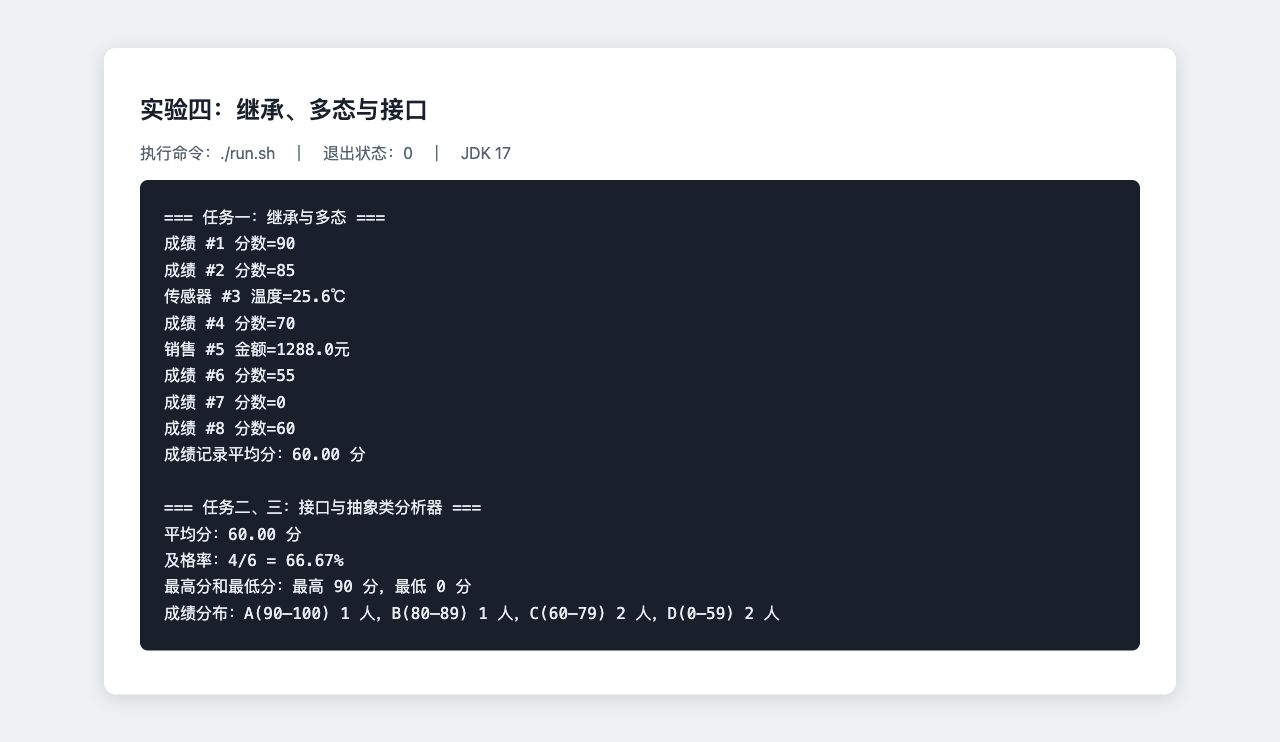
\includegraphics[width=\textwidth]{figure/运行结果截图.png}
  \caption{实际执行程序后的运行结果}
  \label{fig:run}
\end{figure}

六条成绩分别为 90、85、70、55、0 和 60 分。其总和为 360，
平均分为 $360/6=60.00$；最高分为 90，最低分为 0；及格 4 人，
及格率为 $4/6\times 100\%\approx 66.67\%$。
A、B、C、D 四个等级的人数分别为 1、1、2、2，结果与程序输出一致。
补充检查覆盖空数据集、各等级边界、非法成绩、数组复制和动态绑定；
还在独立编译目录中注册额外分析器，验证无需修改主程序即可加载。

\section{思考题}
\subsection{多态如何做到增加子类而不改老代码？}
调用方依赖父类或接口中约定的方法，运行时动态绑定实际对象的重写实现。
例如遍历 \texttt{Record[]} 时只调用 \texttt{summary()}，新增子类实现该方法后，
遍历代码不必修改。这体现了开闭原则：对扩展开放，对已有代码修改关闭。
对象创建或插件注册仍可能需要配置，本实验通过服务文件注册具体分析器。

\subsection{抽象类和接口分别适合什么场景？}
接口适合规定共同能力或调用协议；一个 Java 类可以实现多个接口。
本实验的 \texttt{Analyzer} 规定分析方法，主程序依赖接口处理不同实现。
抽象类适合相关类共享状态和行为；\texttt{BaseAnalyzer} 保存名称并复用输出逻辑，
由具体子类实现分析算法。Java 类只能直接继承一个类，因此接口在组合多种能力时更灵活。

\subsection{父类引用能否调用子类特有方法？}
对于 \texttt{Record r = new ScoreRecord(1, 90)}，不能直接调用
\texttt{r.getScore()}，因为编译器依据引用的声明类型 \texttt{Record} 检查成员，
而该类没有声明 \texttt{getScore()}。\texttt{r.summary()} 则可以调用，
运行时执行子类重写版本。可通过类型检查后向下转型：
\begin{lstlisting}[language=java]
Record r = new ScoreRecord(1, 90);
if (r instanceof ScoreRecord scoreRecord) {
    System.out.println(scoreRecord.getScore());
}
\end{lstlisting}
也可检查后使用 \texttt{((ScoreRecord) r).getScore()}；对不兼容对象直接强制转换会导致
\texttt{ClassCastException}。

\section{实验小结}
本实验完成记录类继承、多态遍历和成绩统计，通过接口统一调用四个分析器，
使用抽象类复用名称与输出逻辑，并通过服务注册验证扩展性。

GitHub 仓库地址：\url{https://github.com/alerk2005-sketch/DataInsight}。
实验源码、运行截图、输出和思考题随报告工程一并提交。
